\section{Obstructed Q-nodes} \label{sec:q_nodes}

Suppose that a Q-node with subtrees $T_1,\dots,T_n$ is obstructed. Then the two possible
orderings of this Q-node are not compatible with $\wlt$. Notice that at most four cliques are
sufficient to create the obstruction. We next prove that at
most three cliques are already sufficient.

\begin{lemma} \label{lem:q_node_three_cliques}
If a Q-node is obstructed, there exists an obstruction created by at most three maximal cliques.
\end{lemma}

\begin{proof}
Suppose that an obstruction is created by four cliques $a \in T_\alpha$, $b \in T_\beta$, $c \in
T_\gamma$ and $d \in T_\delta$ such that $\alpha < \beta$, $\gamma < \delta$, $a \wlt b$, and $c
\wgt d$. We know that $I_a$ is on the left of $I_b$, and $I_c$ is on the right of $I_d$. 
Notice that the four subtrees $T_\alpha$, $T_\beta$, $T_\gamma$ and $T_\delta$ are not necessarily
distinct. We classify all possible orderings $<$ of $\alpha$, $\beta$, $\gamma$, $\delta$ in two
general cases, namely, $\alpha \neq \gamma$ and $\alpha = \gamma$. In the first case, we may assume
without loss of generality that $\alpha < \gamma$.

\emph{Case 1: $\alpha < \gamma < \delta$} (see Fig.~\ref{fig:Q_node_three_cliques}a). Consider the
relative positions of $I_c$ and $I_d$ with respect to $I_a$. If $I_d$ is to the left of $I_a$, we
have $d \wlt a \wlt b$, and these three cliques already create an obstruction. If $I_c$ is to the
right of $I_a$, then we get $a \wlt c$ and $c \wgt d$, creating an obstruction. If neither happens,
then $I_c$ and $I_d$ are subintervals of $I_a$. Thus $c,d \wlt b$. If $\beta \le \gamma$, we have $a
\wlt b$ and $b \wgt d$, creating an obstruction. If $\beta > \gamma$, then $d \wlt c \wlt b$, which
also creates an obstruction.

\begin{figure}[b!]
\centering
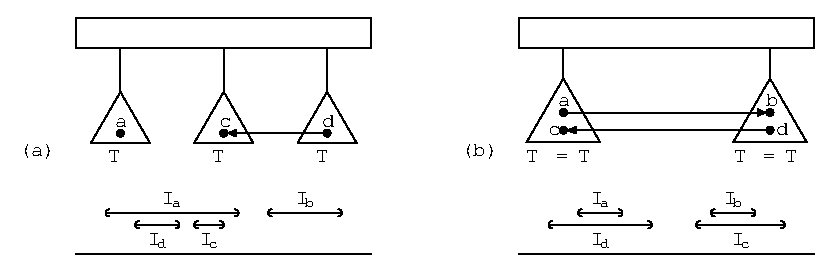
\includegraphics{q_nodes_three_cliques.eps}
\caption{Two cases of the proof of Lemma~\ref{lem:q_node_three_cliques}. The Q-node is depicted in
the top, while in the bottom we have the relative positions of the intervals.}
\label{fig:Q_node_three_cliques}
\end{figure}

\emph{Case 2: $\alpha = \gamma$} (see Fig.~\ref{fig:Q_node_three_cliques}b). If $I_c$ does not
intersect $I_b$, or $I_d$ does not intersect $I_a$, it is easy to see that three of the cliques
already create an obstruction. Suppose next that these intersections occur. Then $d \wlt b$. If
$\delta < \beta$ or $\beta < \delta$, it is again easy to show that three cliques are enough to
create an obstruction. It only remains to consider the case where $\alpha = \gamma < \beta =
\delta$.

Since the intervals $I_c$ and $I_a$ are non-intersecting, we may assume without loss of generality
that there exists $x \in P(a) \setminus P(c)$. This vertex $x$ belongs to sections of $T_\alpha$.
Thus $x \notin P(d)$, and we get that $I_a \subsetneq I_d$. By Lemma~\ref{lem:open_intervals}, $P(d)
\subsetneq P(a)$; in particular, $P(d)$ contains no private pre-drawn interval from sections of
$T_\beta$, and all pre-drawn intervals of $s_\beta(Q)$ are also contained in $s_\alpha(Q)$.

Since $P(d) \setminus P(b) = \emptyset$, there exists $y \in P(b) \setminus P(d)$ which is contained
in sections of $T_\beta$. We next apply the argument in the previous paragraph, and obtain $y \notin
P(c)$, $I_b \subsetneq I_c$, and $P(c) \subsetneq P(b)$. Consequently, $P(c)$ contains no private
pre-drawn intervals from sections of $T_\alpha$, and all pre-drawn intervals of $s_\alpha(Q)$ are
contained in $s_\beta(Q)$. We conclude that $P(c) = P(d)$ and $I_c = I_d$, which gives a
contradiction.\qed
\end{proof}

In summary, we can assume that a minimal obstruction involves at most three maximal cliques.  These
three cliques belong to either two or three different subtrees.

In the rest of the section, many figures describe positions of derived pre-drawn intervals in
sections of the Q-node and its subtrees; for instance Fig.~\ref{fig:Q_node_two_subtrees}. Some of
these intervals necessarily belong to sections of the Q-node, since they belong to maximal cliques
of several subtrees; for instance $t_2$ in Fig.~\ref{fig:Q_node_two_subtrees}. But for the remaining
intervals, it is not important to distinguish whether they belong to sections of the Q-node or one
of its subtrees, only their relative positions in the Q-node matter; for instance $q$ and $x_1$ in
Fig.~\ref{fig:Q_node_two_subtrees}.

\subsection{Cliques in Two Different Subtrees} \label{sec:q_nodes_two_subtrees}

In this section, we deal with the case where the maximal cliques belong to two different subtrees.

\begin{lemma}[The Q-node case, Two Subtrees] \label{lem:q_node_two}
If at most three cliques creating the obstruction belong to two different subtrees, then $G$ and
$\calR'$ contain an SE, $1$-FAT, $2$-FAT, $1$-BI, or $2$-BI obstruction.
\end{lemma}

\begin{proof}
The proof is similar to that of Lemma~\ref{lem:p_node}.  If two maximal cliques create an
obstruction, we can argue as in the first paragraph of the proof of Lemma~\ref{lem:p_node}, and we
obtain an SE obstruction.  It remains to deal with the case of three maximal cliques $a$, $b$, and
$c$.

We can assume that $a \wlt b \wlt c$ and that, for some $i < j$, we have $a,c \in T_i$ and $b \in
T_j$. Furthermore, without loss of generality, there exist $p \in P(a) \setminus P(c)$. Since $p$
belongs to sections of $T_i$, then $p \notin P(b)$, and thus $\inter p'$ lies to the left of $I_b$.
We distinguish two cases. 

\emph{Case 1:} $P(b) \setminus P(c) \ne \emptyset$. Then there exists $q \in P(b) \setminus P(c)$
such that $\inter q'$ lies between $\inter p'$ and $I_c$. Since $q$ is non-adjacent to $p$, it
belongs to sections of either $Q$ or $T_j$. Notice that in any case $s_q^\lft(Q)$ is on the right of
$s_i(Q)$.  Arguing as in Case 1 of the proof of Lemma~\ref{lem:p_node}, we observe that there exists
$r \in P(c) \setminus P(b)$. Furthermore, it follows that $\inter r'$ lies to the right of $\inter
q'$;  see Fig.~\ref{fig:Q_node_two_subtrees}a on the left.

\begin{figure}[b!]
\centering
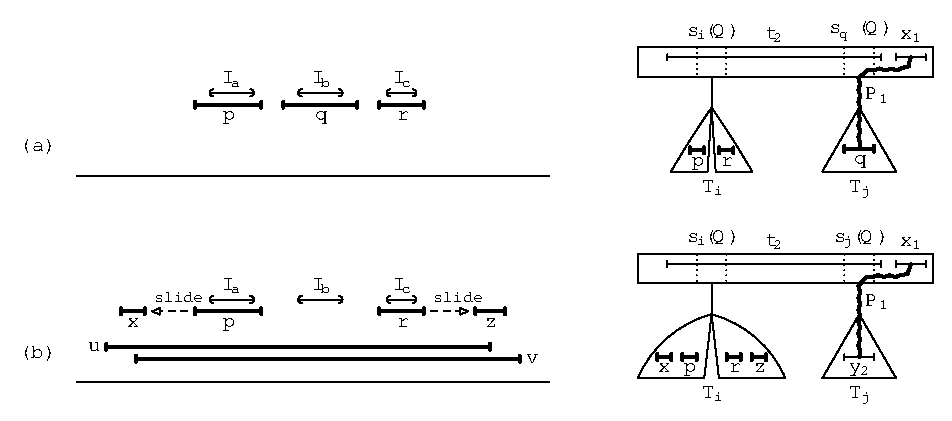
\includegraphics{q_nodes_two_subtrees.eps}
\caption{(a) Case 1: The pre-drawn intervals and the situation in the
MPQ-tree for $s_i(Q) \subsetneq s_q^\lft(Q)$. (b) Case 2: The pre-drawn intervals and the
situation when there exists no path from $x$ to $z$ avoiding the vertices of $b$.}
\label{fig:Q_node_two_subtrees}
\end{figure}

If there exists a path $P_1$ from $p$ to $r$ avoiding $N[q]$, we get a $1$-FAT obstruction for $x_1
= p$, $y_1 = q$, $z_1 = r$ and $P_1$. By Lemma~\ref{lem:different_sections}, we know that $s_i(Q)
\ne s_q^\lft(Q)$. If $s_i(Q) \not\subseteq s_q^\lft(Q)$, then there exists some $w \in s_i(Q)
\setminus s_q^\lft(Q)$. Therefore, $P_1 = pwr$ is such a path. It remains to deal with the case
where no such path $P_1$ exists, which implies that $s_i(Q) \subsetneq s_q^\lft(Q)$; see
Fig.~\ref{fig:Q_node_two_subtrees}a on the right.

Consider the set $W = s_i(Q)$. Let $t_2$ be a vertex of $W$ whose section $s_{t_2}^\rt(Q)$ is
leftmost. Let $C$ be the component of $G[Q] \setminus W$ containing $q$. Since $s_q^\lft(Q)
\setminus W$ is non-empty, $C$ consists of the vertices of at least two subtrees of the Q-node. If
$t_2$ was adjacent to all vertices of $C$, it would be possible to flip the ordering of this
component, contradicting the fact that there are only two possible orderings for $Q$. Therefore,
$t_2$ is not adjacent to all vertices of $C$.  We choose $x_1 \in C \setminus N[t_2]$ whose section
$s_{x_1}^\lft(Q)$ is leftmost.  Let $P_1$ be a shortest path from $q$ to $x_1$ whose inner vertices
are adjacent to $t_2$. It follows that $x_2 = p$, $y_2 = q$, $z_2 = r$, $P_2 = x_2t_2$, $t_2$,
$x_1$, and $P_1$ define a $2$-FAT obstruction. (By Lemma~\ref{lem:monotone_paths}, all inner
vertices of $P_1$ are adjacent to $t_2$.)\qed

\emph{Case 2:} $P(b) \setminus P(c) = \emptyset$. Then there exists $r \in P(c) \setminus P(b)$.
Since $\inter r'$ lies on the right of $I_b$, the vertex $r$ is not contained in $a$ and it belongs
to sections of $T_i$. We use the same approach as in Case 2 of the proof of Lemma~\ref{lem:p_node}.
Since $P(b) \subseteq P(a) \cap P(c)$, every pre-drawn interval of $P(b)$ covers
$[\clql(a),\clqr(c)]$.  Let $u \in P^\endlft(b)$ and $v \in P^\startrt(b)$ (possibly $u=v$).

By applying Sliding Lemma~\ref{lem:sliding} twice, we get $x,z \notin P(b)$ such that $\inter x'$
covers $\ell(v)$ and $\inter z'$ covers $r(u)$; see Fig.~\ref{fig:Q_node_two_subtrees}b on the left.
Suppose that there exists a path $P_{x,z}$ from $x$ to $z$ avoiding all vertices of $b$. Let $x_1 =
x$, $z_1 = z$, and $P_1$ be a shortest path from $x_1$ to $z_1$ in $G[Q] \setminus b$.
By Lemma~\ref{lem:non_adjacent}, there exists $y_1 \in b$ non-adjacent to $P_1$. We
obtain a $1$-BI obstruction.

Suppose next that there is no path $P_{x,z}$ avoiding $b$.  We know that $x$ and $y$ belong to
sections of $T_i$, since there exist paths $P_{x,p}$ and $P_{r,z}$ avoiding $b$, from the above
applications of Sliding Lemma~\ref{lem:sliding}.  Since no path $P_{x,z}$ avoiding $b$ exists, we
have $s_i(Q) \subsetneq s_j(Q)$.  As in Case 1, let $W = s_i(Q)$, and let $t_2$ be a vertex of $W$
whose section $s_{t_2}^\rt(Q)$ is leftmost (possibly $t_2 = u$ or $t_2 = v$).  We again infer that
$t_2$ is not adjacent to all vertices of $C$, where $C$ is the component of $G[Q] \setminus W$
containing $b \setminus W$. We choose $x_1 \in C \setminus N[t_2]$ whose section $s_{x_1}^\lft(Q)$
is leftmost. Since $s_i(Q) \subsetneq s_j(Q) \subseteq b$, there exists $y_2 \in b$ non-adjacent to
$x$ and $z$. We get a 2-BI obstruction for $x_2 = x$, $y_2$, $z_2 = z$, $u$, $v$, a shortest path
$P_1$ from $y_2$ to $x_1$ in $C$, and $P_2 = x_2t_2$. (By Lemma~\ref{lem:monotone_paths}, all inner
vertices of $P_1$ are adjacent to $t_2$.)\qed
\end{proof}

\subsection{$k$-FAT and $(k,\ell)$-CE Lemmas} \label{sec:q_nodes_k_fat}

In this section, we give two tools for the case, analyzed in
Section~\ref{sec:q_nodes_three_subtrees}, where the three maximal cliques creating the obstruction belong to
three different subtrees. These tools give insight into the structure of the Q-nodes, and explain
the way in which complex obstructions such as $k$-FAT and $(k,\ell)$-CE obstructions are formed.

\heading{$\boldsymbol k$-FAT Lemma.} First, we present a useful lemma that allows to locate $k$-FAT
obstructions. The key idea of the proof is similar to Case 1 of the proof of
Lemma~\ref{lem:q_node_two}, but applied inductively for $k$. 

\begin{lemma}[$\boldsymbol k$-FAT] \label{lem:k_fat}
Let $Q$ be a Q-node with children $T_1,\dots,T_n$, and let $a$, $b$ and $c$ be three cliques of
$T[Q]$ contained respectively in $T_\alpha$, $T_\beta$ and $T_\gamma$, for $\alpha < \beta < \gamma$.
Let $x_k \in P(a)$, $y_k \in P(c)$ and $z_k \in P(b)$ be three disjoint pre-drawn intervals such
that $\inter{y_k}'$ is between $\inter{x_k}'$ and $\inter{z_k}'$. Then $G[Q]$ and
$\calR'[\{x_k,y_k,z_k\}]$ contain a $k$-FAT obstruction.
\end{lemma}

\begin{proof}
The proof, illustrated in Fig.~\ref{fig:q_nodes_k_fat_statement}, is by induction. We always denote
the vertices as in the definition of $k$-FAT obstructions. If we find a $1$-FAT or $2$-FAT
obstruction, the statement is true.  Otherwise, we recurse on a smaller part of the Q-node, where we
find a structure identical to a $(k-1)$-FAT obstruction, except for the fact that the vertex
$x_{k-1}$ is free. Together with some vertices in the remainder of the Q-node, we obtain a $k$-FAT
obstruction. We next provide the details.

\begin{figure}[b!]
\centering
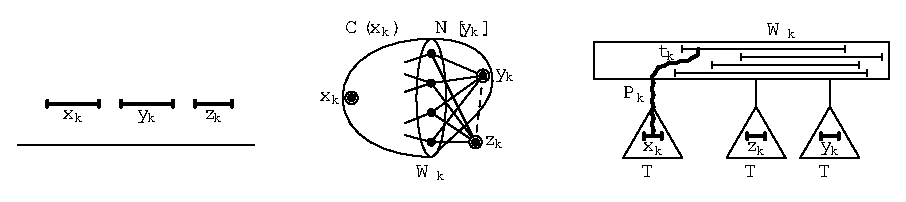
\includegraphics{q_nodes_k_fat_statement.eps}
\caption{On the left, the position of the pre-drawn intervals.  In
the middle, the construction of $W_k \subsetneq N[y_k]$ in $G[Q]$. On the right, the Q-node with the
three subtrees and the intervals of $W_k$ depicted in its sections.}
\label{fig:q_nodes_k_fat_statement}
\end{figure}

Let $k$ be some yet unspecified integer, determined by the recursion. We want to argue that $G[Q]$
contains a $k$-FAT obstruction because the ordering of $\inter{x_k}'$, $\inter{y_k}'$ and
$\inter{z_k}'$ is incorrect (in every representation, $\inter{z_k}$ is between $\inter{x_k}$ and
$\inter{y_k}$). Suppose that there exists a path from $x_k$ to $z_k$ whose inner vertices are
non-adjacent to $y_k$. Then we obtain a $1$-FAT obstruction. It remains to deal with the harder
situation where no such path exists.

Let $C(x_k)$ be the connected component of $G[Q] \setminus N[y_k]$ containing $x_k$. By our
assumption, $z_k \notin C(x_k)$. We denote by $W_k$ the subset of $N[y_k]$ containing those vertices
that are adjacent to some vertex of $C(x_k)$; see Fig.~\ref{fig:q_nodes_k_fat_statement}, middle.
Notice that the vertices of $C(x_k)$ appear only in sections and subtrees to the left of
$s_\beta(Q)$.  Therefore, every vertex of $W_k$ lies in the sections of $Q$ and stretches from the
left of $s_\beta(Q)$ to $s_\gamma(Q)$; see Fig.~\ref{fig:q_nodes_k_fat_statement}, right. In other
words, $W_k \subseteq s_\beta(Q) \cap s_\gamma(Q)$ and every vertex of $W_k$ is adjacent to $z_k$.

Let $C$ be a connected component of $G[Q] \setminus W_k$. If $C$ contains a vertex from some section
of $Q$, we call it \emph{big}. Notice that in this situation $C$ has a vertex contained in two
consecutive sections of $Q$ and their subtrees. Otherwise, $C$ consists of some vertices of a
subtree of $Q$, and we call it \emph{small}. The section above a subtree containing a small
component is a subset of $W_k$. Additionally, if two small components are placed in two different
subtrees, the two sections above these subtrees are different.

The graph $G[Q] \setminus W_k$ is disconnected, as $x_k$ and $z_k$ belong to different
components. Let us denote the connected component containing $y_k$ by $C(y_k)$, and the one
containing $z_k$ by $C(z_k)$.  
Let $t_k$ be a vertex of $W_k$ whose section
$s_{t_k}^\rt(Q)$ is leftmost. Let $P_k$ be a shortest path from $x_k$ to $t_k$ in $G[C(x_k) \cup \{t_k\}]$; see
Fig.~\ref{fig:q_nodes_k_fat_statement}, right. We distinguish two cases.

\begin{figure}[t!]
\centering
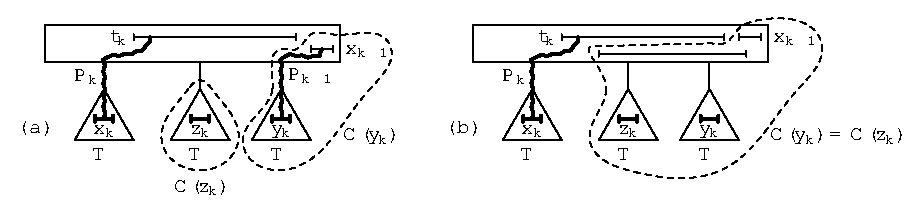
\includegraphics{q_nodes_k_fat_two_cases.eps}
\caption{(a) In Case 1, there exists a path $P_{k-1}$ from $x_{k-1}$ to $y_k$ whose inner
vertices avoid $z_k$. (b) In Case 2, we have
$C(y_k) = C(z_k)$ and such a path might no longer exist. For instance, every path from $x_{k-1}$ to
$y_k$ in $C(y_k)$ might use the depicted interval in the sections of $Q$, which is also
adjacent to $z_k$.}
\label{fig:q_nodes_k_fat_two_cases}
\end{figure}

\emph{Case 1: $C(y_k) \ne C(z_k)$.} This case is very similar to the proof of
Lemma~\ref{lem:q_node_two}; see Fig.~\ref{fig:q_nodes_k_fat_two_cases}a. Every vertex of $W_k$ is
adjacent to some vertex of $C(x_k)$ and to some vertex of $C(y_k)$. Therefore, it is also adjacent
to every vertex of $C(z_k)$. If $C(z_k)$ was big, then we could reverse its sections in the Q-node,
contradicting the fact that there are only two possible orderings for a Q-node. Therefore, $C(z_k)$
is small. Notice that then $C(y_k)$ is not small, since otherwise we would get $s_\beta(Q) = W_k =
s_\gamma(Q)$, contradicting Lemma~\ref{lem:different_sections}. Thus, $C(y_k)$ is big.

Let us set $y_{k-1} = z_k$ and $z_{k-1} = y_k$. The vertex $t_k$ is not universal for $C(y_k)$;
otherwise, every vertex of $W_k$ would be universal and this would give additional orderings of
$C(y_k)$ in $Q$.  Let $x_{k-1}$ be a vertex of $C(y_k) \setminus N[t_k]$ whose section
$s_{x_{k-1}}^\lft(Q)$ is leftmost. Notice that $s_{x_{k-1}}^\lft(Q)$ is always the next section to
$s_{t_k}^\rt(Q)$. Let $P_{k-1}$ be a shortest path from $x_{k-1}$ to $z_{k-1}$ in $C(y_k)$. By
Lemma~\ref{lem:monotone_paths}, all inner vertices of $P_{k-1}$ are adjacent to $t_k$.  Since this
path lies in $C(y_k)$, the inner vertices are non-adjacent to $y_{k-1}$, $x_k$ and $P_k$. We have
constructed a $2$-FAT obstruction.

\emph{Case 2: $C(y_k) = C(z_k)$.} In this case, the component $C(y_k)$ is big; see
Fig.~\ref{fig:q_nodes_k_fat_two_cases}b. Therefore, similarly as above, $t_k$ is not universal for
$C(y_k)$. We put $y_{k-1} = z_k$ and $z_{k-1} = y_k$. We choose $x_{k-1} \in C(y_k) \setminus
N[t_k]$ in the same way as in Case 1.  Notice that $x_{k-1}$ is a non-neighbor of $y_{k-1}$, since
otherwise it would be a neighbor of $t_k$.  On the other hand, $x_{k-1}$ might be adjacent to
$z_{k-1}$ or not. If it is, we get a $2$-FAT obstruction for $k=2$ with $P_1 = x_{k-1}z_{k-1}$. If
it is not, we proceed as follows.
	
As before, every shortest path from $x_{k-1}$ to $z_{k-1}$ has all inner vertices adjacent to $t_k$.
Since all vertices of $C(y_k)$ are non-adjacent to $x_k$ and the inner vertices of $P_k$, every
shortest path satisfies this as well.  There exists a shortest path from $x_{k-1}$ to
$z_{k-1}$ in $C(y_k)$, but we cannot guarantee that the inner vertices of this path are non-adjacent
to $y_{k-1}$. We solve this issue by applying the entire argument of the proof recursively to
$C(y_k)$.

In every representation extending the partial representation, the intervals of $C(x_k)$ form a
connected subset of the real line placed to the left of $\inter{y_k}'$. Therefore, $\inter{t_k}$
stretches from $C(x_k)$ to $\inter{z_k}'$, covering $\inter{y_k}'$. Thus $\inter{x_{k-1}}$ is placed
to the right of $\inter{z_k}' = \inter{y_{k-1}}'$ in every extending representation (see
Fig.~\ref{fig:k_FAT}b).  Again, $\inter{y_{k-1}}'$ has to be placed between $\inter{x_{k-1}}$ and
$\inter{z_{k-1}}'$. We assume that $\inter{x_{k-1}}$ is pre-drawn on the right of $\inter{y_{k-1}}'$
and repeat the same argument for $C(y_k)$ and the MPQ-tree restricted to these vertices. The role of
$x_k$, $y_k$ and $z_k$ is played by $x_{k-1}$, $y_{k-1}$ and $z_{k-1}$, respectively. (The ordering
of the pre-drawn intervals is flipped.)

The paragraphs above show the induction step of our proof (by induction on, say, the number of
considered sections of $Q$). By the induction hypothesis, we find a $(k-1)$-FAT obstruction.  By
making $x_{k-1}$ free and adding $x_k$, $t_k$ and $P_k$, we get a $k$-FAT obstruction in the
original partial representation.  Clearly $t_k$ is adjacent to the entire $(k-1)$-FAT obstruction
with the exception of $x_{k-1}$, since all further vertices are contained in a section to the left
of $s_{x_{k-1}}^\lft(Q)$. The reason is that we always use shortest paths which are $Q$-monotone by
Lemma~\ref{lem:monotone_paths}.  By the same reason, they are non-adjacent to the inner vertices of
$P_k$ and to $x_k$, as required.

To make the argument complete, we should check that all the assumptions used throughout the proof
apply recursively, in particular the arguments concerning non-universality of $t_{k-1}$ and
reversing big components. This is true because both components $C(y_{k-1})$ and $C(z_{k-1})$ of
$C(y_k) \setminus W_{k-1}$ appear to the left of $x_{k-1}$, so $t_k$ and the other vertices of $W_k$
are universal for them. This property is preserved throughout the recursion, so $C(y_\ell)$ and
$C(z_\ell)$ are adjacent to all vertices of $W_k,W_{k-1},\dots,W_{\ell+1}$. Similarly,
the rest of the inductive proof can be formalized.\qed
\end{proof}

\begin{figure}[t!]
\centering
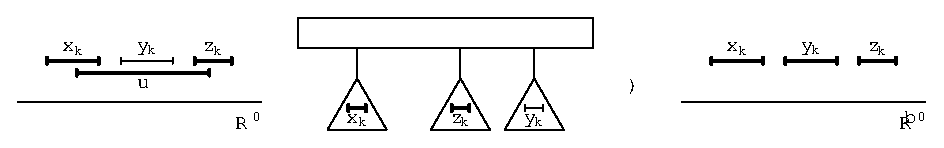
\includegraphics{q_nodes_using_k_fat.eps}
\caption{Suppose that we show that a partial representation $\calR'$ has three pre-drawn intervals
as on the left, and that there is a vertex $y_k$ adjacent to $u$ and non-adjacent to $x_k$ and
$z_k$. Then $\inter{y_k}$ has to be placed between $\inter{x_k}'$ and $\inter{z_k}'$ in every
extending representation. Thus, we can assume it is pre-drawn there and obtain a modified partial
representation $\widehat\calR'$. If we further show that $x_k$, $y_k$ and $z_k$ are placed in
appropriate sections of $G[Q]$ for some Q-node $Q$, we can apply $k$-FAT Lemma~\ref{lem:k_fat} and
we get a $k$-FAT obstruction in $G[Q]$ and $\widehat\calR'[\{x_k,y_k,z_k\}]$. Together with $\inter
u'$, this forms a $k$-BI obstruction in $G$ and $\calR'$.}
\label{fig:q_nodes_using_k_fat}
\end{figure}

The above proof shows that the structure of a Q-node can be highly complicated, leading to 
complicated obstructions such as $k$-FAT. Actually, $k$-FAT Lemma~\ref{lem:k_fat} is a very useful tool
because it can be also applied in situations where not all
$x_k$, $y_k$, and $z_k$ are pre-drawn, to build other obstructions.
Fig.~\ref{fig:q_nodes_using_k_fat} shows an example.

\begin{lemma} \label{lem:k_fat_contains_1_fat}
Consider a $k$-FAT obstruction $H_k$ for $k>2$. If we swap the positions of $\inter{x_k}'$ and
$\inter{y_k}'$, then we obtain a new obstruction which contains a $1$-FAT obstruction for $x'_1 =
y_k$, $y'_1 = x_k$, and $z'_1 = z_k$. Further, if $k=2$ and this does not happen, then $x_2$ is
adjacent to $t_2$.
\end{lemma}

\begin{proof}
For $k \ge 3$, the graph $H_k \setminus N[x_k]$ is connected; in particular, there
exists a path $P'_1 = y_kt_{k-1}z_k$ avoiding $N[x_k]$. For $k=2$, there exists a path $P'_1 =
y_2t_2z_2$ avoiding $N[x_2]$, unless $x_2$ is adjacent to $t_2$.\qed
\end{proof}

\heading{$\boldsymbol{(k,\ell)}$-CE Lemma.} Suppose that we have the situation in
Fig.~\ref{fig:q_nodes_kl_ce_statement}. We can easily show that there is some $(k,\ell)$-CE
obstruction by applying $k$-FAT Lemma~\ref{lem:k_fat} twice, once when $\inter{x_k}$ is on the left
of $\inter{y_k}$ and once when it is on the right.  The following lemma reveals its structure in
detail.

\begin{figure}[b!]
\centering
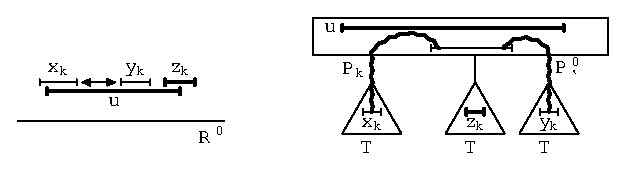
\includegraphics{q_nodes_kl_ce_statement.eps}
\caption{When $\inter u'$ single overlaps $\inter{z_k}'$, and the vertices $x_k$, $y_k$, and $z_k$ are
placed in the MPQ-tree as on the right, we get a $(k,\ell)$-CE obstruction.}
\label{fig:q_nodes_kl_ce_statement}
\end{figure}

\begin{lemma}[$(\boldsymbol{k},\boldsymbol{\ell})$-CE] \label{lem:kl_ce}
Let $Q$ be a Q-node with children $T_1,\dots,T_n$, and let $a$, $b$ and $c$ be three cliques of
$T[Q]$ contained respectively in $T_\alpha$, $T_\beta$ and $T_\gamma$, for $\alpha < \beta < \gamma$.
Let $x_k \in a$, $y_k \in c$ and $z_k \in P(b)$ be three non-adjacent vertices having a common
pre-drawn neighbor $u$ such that $\inter{u}'$ single overlaps $\inter{z_k}'$.
Then $G[Q] \cup \{u\}$ and $\calR'[\{z_k,u\}]$ contain a $(k,\ell)$-CE obstruction, where either $\ell=1$ or
$k = \ell = 2$.
\end{lemma}

\begin{proof}
The simplest case is when there exist a path $P_k$ from $x_k$ to $z_k$ avoiding $N[y_k]$, and a path
$P_\ell'$ from $y_k$ to $z_k$ avoiding $N[x_k]$. Let $P_k$ and $P_\ell'$ be shortest such paths as
in Fig.~\ref{fig:q_nodes_kl_ce_statement}, right. We get a $(1,1)$-CE obstruction. By
Lemma~\ref{lem:monotone_paths}, the paths $P_k$ and $P_\ell'$ are monotone. Therefore, their inner
vertices are non-adjacent to each other, with the possible exception of the last vertices before
$z_k$, which can be adjacent or even identical. Concerning minimality, we can always find one of the
three finite $(1,1)$-CE obstructions depicted in Fig.~\ref{fig:kl_CE_obstructions}a. The reason is
that when paths $P_k$ and $P'_\ell$ are long, we can take as $x_k$ and $y_k$ one of their inner
vertices, making them shorter.

Suppose next that there exists no path $P_k$ from $x_k$ to $z_k$ avoiding $N[y_k]$.  Let $C(x_k)$,
$W_k$, and $t_k$ be defined as in the proof of $k$-FAT Lemma~\ref{lem:k_fat}. Following the argument
in that proof, we get the subgraph $H_k$ of a $k$-FAT obstruction, which is not the complete $k$-FAT
obstruction because $x_k$ and $y_k$ are free. 

\emph{Case 1: There exists some path $P_\ell'$ from $y_k$ to $z_k$ avoiding $N[x_k]$.} Let $P'_\ell$
be a shortest such path (notice that $\ell = 1$). Together with the above subgraph $H_k$, we get a $(k,1)$-CE
obstruction; see Fig.~\ref{fig:q_nodes_kl_ce_two_cases}a. In particular, if some vertex $w \in W_k$
is non-adjacent to $x_k$ (possibly $w = t_k$), we can use $P'_\ell = y_kwz_k$. 

We note that when $k \ge 3$, such a path $P_\ell'$ necessarily exists, as we can use $P'_\ell =
y_kt_{k-1}z_k$, as argued in Lemma~\ref{lem:k_fat_contains_1_fat}. Therefore, the $(k,1)$-CE
obstructions consist of the subgraph $H_k$ together with $u$; assuming minimality, we have that
either $u$ is adjacent to all vertices of $H_k$, or $u = t_k$.  If $k = 2$, then $P_\ell'$ might
still exist but it might be longer and might use inner vertices not contained in $H_k$. Concerning
minimality, we always find one of the three $(2,1)$-CE obstructions depicted in
Fig.~\ref{fig:kl_CE_obstructions}b. Indeed, $P_2$ can be assumed to be of length one or two, since
otherwise we could use one of its inner vertices as $x_2$. For length two, we get $P'_1 =
y_kt_kz_k$. For length one, we get a path $P'_1$ from $z_2$ to $y_2$, and we can assume that $y_2$
is adjacent to $x_1$ (otherwise we could use as $y_2$ the neighbor of $x_1$ on $P_1$).

\begin{figure}[t!]
\centering
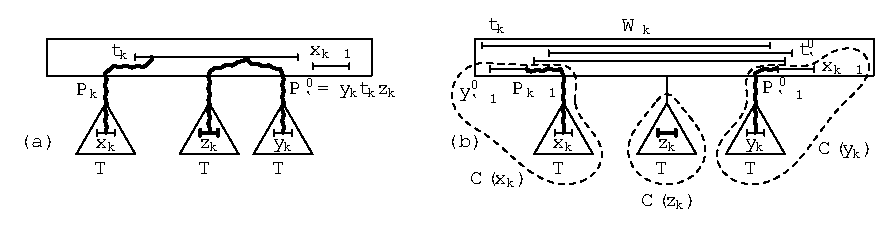
\includegraphics{q_nodes_kl_ce_two_cases.eps}
\caption{(a) Case 1: If there exists a path $P'_\ell$ from $y_k$ to $z_k$ avoiding $N[x_k]$, then we get a
$(k,1)$-CE obstruction. (b) Case 2: We get a $(2,2)$-CE obstruction.}
\label{fig:q_nodes_kl_ce_two_cases}
\end{figure}

\emph{Case 2: No such path $P'_\ell$ exists.}
By Lemma~\ref{lem:k_fat_contains_1_fat}, $k = 2$.
We want to show that there exists a $(2,2)$-CE obstruction. 

Notice that all vertices $w\in W_k$ are
adjacent to $x_k$, $y_k$, and $z_k$, since otherwise there would exist a path $P'_\ell = y_kwz_k$.
Hence the vertices of $W_k$ belong to sections of $Q$, covering all subtrees between $T_\alpha$ and
$T_\gamma$; see Fig.~\ref{fig:q_nodes_kl_ce_two_cases}b. Let $C(y_k)$ and $C(z_k)$ be the components
of $G[Q] \setminus W_k$ containing $y_k$ and $z_k$, respectively.  Since there exists no path
$P'_\ell$, we obtain that $C(x_k)$, $C(y_k)$, and $C(z_k)$ are pairwise different.  To determine the
structure of a $(2,2)$-CE obstruction, we apply the argument from Case 1 of the proof of
$k$-FAT Lemma~\ref{lem:k_fat} symmetrically twice.

Let $t_k$ be a vertex of $W_k$ having leftmost section $s_{t_k}^\rt(Q)$ and let $t'_\ell$ be a
vertex of $W_k$ having rightmost section $s_{t'_\ell}^\lft(Q)$ (possibly $t_k = t'_\ell$).  It is
easy to see that $C(z_k)$ is small, otherwise we could flip it and obtain an
ordering of the maximal cliques not compatible with the Q-node.

Similarly as in the proof of $k$-FAT Lemma~\ref{lem:k_fat}, this implies that both $C(x_k)$ and
$C(y_k)$ are big. Therefore, $t_k$ is not universal for $C(y_k)$ and $t'_\ell$ is not universal for
$C(x_k)$. As in the proof of $k$-FAT Lemma~\ref{lem:k_fat}, we choose $x_{k-1} \in C(y_k)$
non-adjacent to $t_k$  and $y'_{\ell-1} \in C(x_k)$ non-adjacent to $t'_\ell$.  There exist paths
$P_{k-1}$ from $x_{k-1}$ to $y_k$ and $P'_{\ell-1}$ from $y'_{\ell-1}$ to $x_k$.  In consequence, we
obtain a $(2,2)$-CE obstruction.

Regarding minimality, notice that we can assume that $y_2$ is adjacent to $x_1$, and $x_2$ is adjacent to $y'_1$;
otherwise, we could choose as $y_2$ and $x_2$ the neighbors of $x_1$ and $y'_1$ on the paths $P_1$ and
$P'_1$, respectively. We get the four minimal finite $(2,2)$-CE obstructions that are illustrated in
Fig.~\ref{fig:kl_CE_obstructions}c.
\qed
\end{proof}

\begin{figure}[t!]
\centering
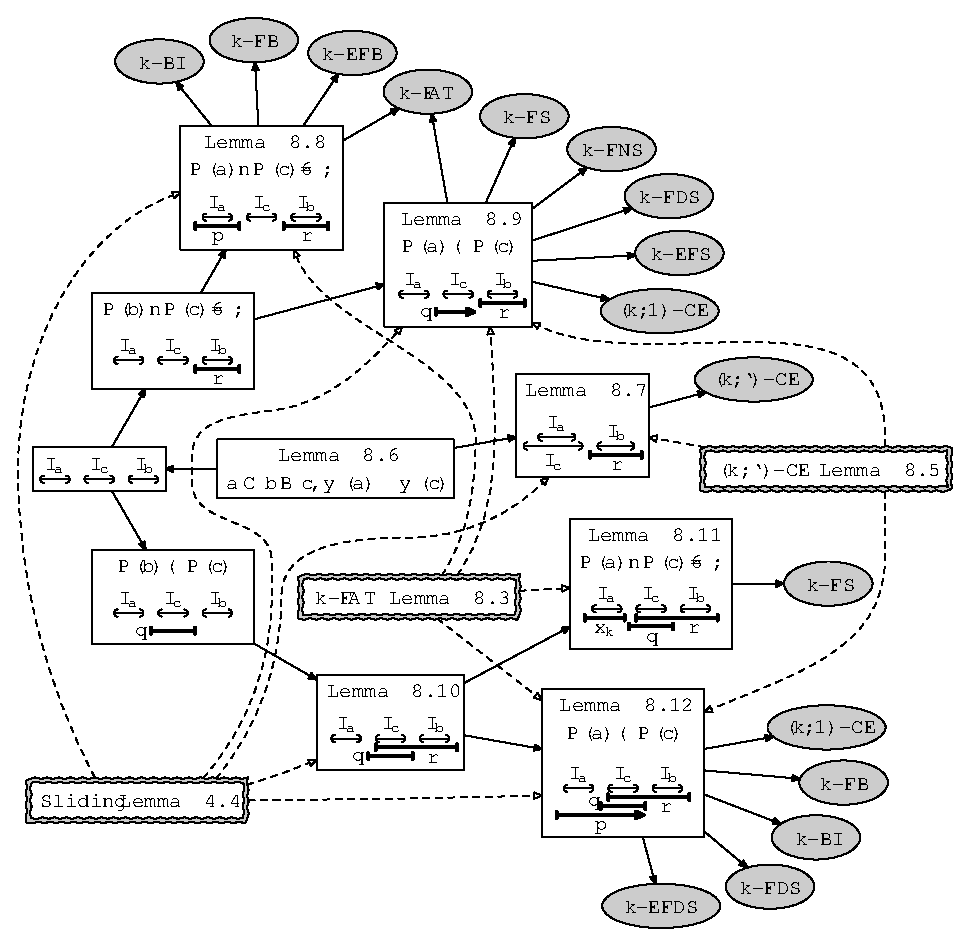
\includegraphics{q_nodes_three_subtrees_diagram.eps}
\caption{A summary of Section~\ref{sec:q_nodes_three_subtrees}. The diagram starts in the middle with
Lemma~\ref{lem:q_node_wlog_lemma}. Inside the cases, we draw the positions of $I_a$, $I_b$, $I_c$,
and some pre-drawn intervals. An arrow at a pre-drawn interval means that it may be further
stretched in the given direction.  The obtained obstructions are highlighted in gray, the used tools
have highlighted borders.}
\label{fig:q_nodes_three_subtrees_diagram}
\end{figure}

\subsection{Cliques in Three Different Subtrees} \label{sec:q_nodes_three_subtrees}

When a Q-node $Q$ is obstructed by three maximal cliques $a \in T_\alpha$, $b \in T_\beta$ and
$T_\gamma$, where $\alpha < \beta < \gamma$, the situation is quite complex.
Fig.~\ref{fig:q_nodes_three_subtrees_diagram} gives an overview of the cases and obstructions
obtained in this case. 

\begin{lemma} \label{lem:q_node_wlog_lemma}
Without loss of generality, we can assume that $a \wlt b \wgt c$ and $\clqr(a) \le \clqr(c)$.
\end{lemma}

\begin{proof}
Since $a$, $b$ and $c$ create an obstruction, $b$ is either a minimal or a maximal element in $\wlt
|_{\{a,b,c\}}$. Without loss of generality (using the flip operation), we can assume that $b$ is
maximal, so $a \wlt b \wgt c$.  Since we can swap $a$ and $c$ by reversing the Q-node, we can assume
that $\clqr(a) \le
\clqr(c)$.\qed
\end{proof}

Since $a \wlt b \wgt c$, both $I_a$ and $I_c$ appear on the left of $I_b$.  Since $\clqr(a) \le
\clqr(c)$, either $I_a$ contained in $I_c$, or $I_a$ is on the left of $I_c$. The first case is easier:

\begin{lemma} \label{lem:q_node_containment_case}
If $I_a$ is contained in $I_c$, then $G$ and $\calR'$ contain a $(k,\ell)$-CE obstruction, where
$\ell = 1$ or $2 \ge k \ge \ell$.
\end{lemma}

\begin{proof}
The proof is illustrated in Fig.~\ref{fig:q_nodes_containment_case}.  By
Lemma~\ref{lem:open_intervals}, $P(c) \subseteq P(a)$. Since $b$ is placed between $a$ and $c$ in
the Q-node $Q$, every vertex contained in both $a$ and $c$ is contained in $b$ as well. Hence $P(c)
\subsetneq P(b)$, and there exists $r \in P(b) \setminus P(c)$. Since $\inter r'$ is on the right of
$I_c$, it is also on the right of $I_a$, and thus $r \notin P(a)$.

Let $u \in P^{\endlft}(c)$. We apply Sliding Lemma~\ref{lem:sliding} to $I_c$, $I_b$, and $\inter
r'$. We get a pre-drawn interval $\inter{z_k}'$ covering $r(u)$, and an induced path $P_{r,z_k}$
from $r$ to $z_k$ consisting of pre-drawn intervals not in $P(c)$. Therefore $z_k$ is on the left of
$c$ in $Q$. Since all pre-drawn intervals of $P_{r,z_k}$ do not belong to $P(c)$, they are on the
right of $I_c$. Thus they are also on the right of $I_a$, which implies that they do not belong to
$P(a)$. Consequently, $z_k$ is between $a$ and $c$ in $Q$.

\begin{figure}[t!]
\centering
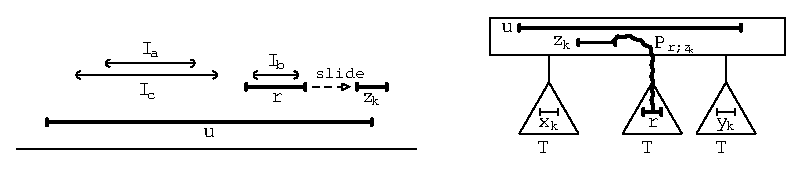
\includegraphics{q_nodes_containment_case.eps}
\caption{Proof of Lemma~\ref{lem:q_node_containment_case}. On the left, the pre-drawn
intervals. On the right, their positions in the MPQ-tree.}
\label{fig:q_nodes_containment_case}
\end{figure}

Let $x_k \in a$ and $y_k \in c$ be vertices non-adjacent to $z_k$. By $(k,\ell)$-CE
Lemma~\ref{lem:kl_ce}, $x_k$, $y_k$, $z_k$, and $u$ create a $(k,\ell)$-CE obstruction, for $\ell =
1$ or $2 \ge k \ge \ell$. Notice that the clique associated to $z_k$ is some $b'\neq b$.\qed
\end{proof}

The case where $I_a$ is on the left of $I_c$ is further divided into several subcases. In the next two lemmas, we focus on the situation where $P(b) \setminus P(c) \ne \emptyset$.

\begin{lemma} \label{lem:q_node_p_and_r_case}
If $I_a$ is on the left of $I_c$, $P(b) \setminus P(c) \ne \emptyset$ and $P(a) \setminus P(c) \ne
\emptyset$, then $G$ and $\calR'$ contain a $k$-FAT, $k$-BI ($k \le 2$), $k$-FB, or $k$-EFB
obstruction.
\end{lemma}

\begin{proof}
The proof is illustrated in Fig.~\ref{fig:q_nodes_p_and_r_case}.  Let $p \in P(a) \setminus P(c)$ and
$r \in P(b) \setminus P(c)$. Then $\inter p'$ is on the left of $I_c$, and $\inter r'$ is on the
right of $I_c$.  Clearly, $\inter p'$ and $\inter r'$ are disjoint, so $p$ appears in the Q-node on
 the left of $r$. Let $u \in P^{\endlft}(c)$ and $v \in P^{\startrt}(c)$ (possibly $u = v$).

\begin{figure}[b!]
\centering
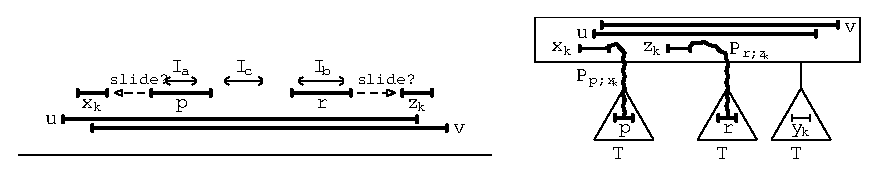
\includegraphics{q_nodes_p_and_r_case.eps}
\caption{Proof of Lemma~\ref{lem:q_node_p_and_r_case}. On the left, the pre-drawn
intervals, with possible sliding on each side. On the right, their positions in the MPQ-tree.}
\label{fig:q_nodes_p_and_r_case}
\end{figure}

If $r(u) \le r(r)$, then $z_k = r$. Obviously, $z_k$ is between $p$ and $c$ in the Q-node.
Otherwise, $P(c) \subsetneq P(b)$, and we apply Sliding Lemma~\ref{lem:sliding} to $I_c$, $I_b$, and
$r$. We obtain a pre-drawn interval $\inter{z_k}'$ not contained in $P(c)$ covering $r(u)$, and a
path $P_{r,z_k}$ whose inner vertices are pre-drawn and not contained in $P(c)$. Notice that all of
these pre-drawn vertices are on the right of $I_c$.  Therefore, these vertices are not contained in
$P(a)$. In this case, we also get that $z_k$ is between $p$ and $c$ in the Q-node.  

Similarly, if $\ell(p) \le \ell(v)$, then $x_k = p$. Otherwise, we use the flipped version of
Sliding Lemma~\ref{lem:sliding} to $I_c$, $I_a$, and $p$, which gives a pre-drawn interval
$\inter{x_k}'$ not contained in $P(c)$ covering $\ell(v)$. By a similar argument, in both cases, we
show that $x_k$ is on the left of $z_k$ in the Q-node.

Let $y_k \in c$ be a vertex non-adjacent to $z_k$ (possibly, $y_k = u$ or $y_k = v$).  Such a vertex
exists because $z_k$ is on the left of $c$ in the Q-node. Notice that $y_k$ is also non-adjacent to
$x_k$. Since $y_k$ is adjacent to $u$ and $v$, in every extending representation $\inter{y_k}$ is
between $\inter{x_k}'$ and $\inter{z_k}'$. So we can assume that it is pre-drawn in this position
and, by $k$-FAT Lemma~\ref{lem:k_fat}, we get a $k$-FAT obstruction. Together with $u$ and $v$ (or
possibly only one of them), we get one of the obstructions in
Fig.~\ref{fig:q_nodes_p_and_r_case_obstructions}.\qed

\begin{figure}[t!]
\centering
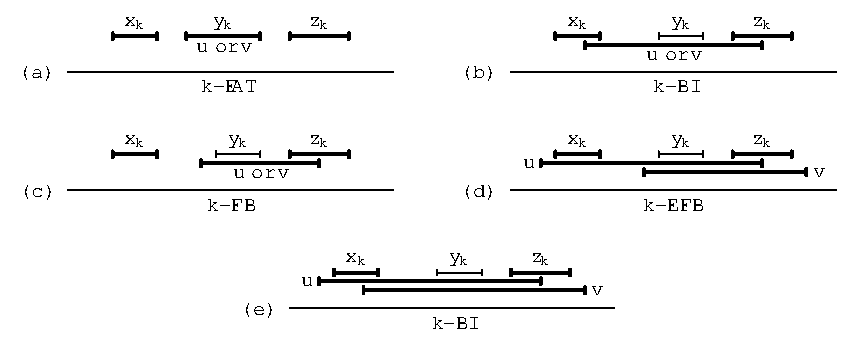
\includegraphics{q_nodes_p_and_r_case_obstructions.eps}
\caption{The different obstructions obtained in the proof of Lemma~\ref{lem:q_node_p_and_r_case}.
If $\ell(x_k) \le \ell(u) \le r(u) \le r(z_k)$, we get one of the obstructions (a) to (c). Since
$z_k$ is in the Q-node between $x_k$ and $c$, if $u$ or $v$ intersect $x_k$, then they also
intersect $z_k$. In the cases (d) and (e), $\ell(u) < \ell(x_k)$ and $r(z_k) < r(v)$. Since $u$
intersects $z_k$, there are only two possible obstructions.}
\label{fig:q_nodes_p_and_r_case_obstructions}
\end{figure}

\end{proof}

\begin{lemma} \label{lem:q_node_q_and_r_case}
If $I_a$ is on the left of $I_c$, $P(b) \setminus P(c) \ne \emptyset$ and $P(a) \subsetneq
P(c)$, then $G$ and $\calR'$ contain a $k$-FAT, $(k,1)$-CE, $k$-FS, $k$-FDS, $k$-FNS, or $k$-EFS obstruction.
\end{lemma}

\begin{proof}
We choose $r \in P(b) \setminus P(c)$ and $q \in P(c) \setminus P(a)$ with leftmost right endpoint.
Then $\inter r'$ is on the right of $I_c$ and $\inter q'$ is on the right of $I_a$.  We note that
$q$ might be adjacent to $r$ or not, and might belong to $P(b)$ or not. Since $P(a) \subsetneq
P(c)$, we get from the structure of the Q-node that also $P(a) \subsetneq P(b)$.  Let $u \in
P^{\endlft}(a)$. Notice that at least one of $q$ and $u$ belongs to $P^{\endlft}(c)$. 

\emph{Case 1: $u \in P^{\endlft}(c)$}. Then $r(u) \le r(q)$ and $P(c) \subsetneq P(b)$; the
situation is depicted in Fig.~\ref{fig:q_nodes_q_and_r_case}a.  We apply Sliding
Lemma~\ref{lem:sliding} to $I_c$, $I_b$, and $r$. We get a pre-drawn interval $z_k \notin P(c)$
covering $r(u)$, and a path $P_{r,z_k}$ consisting of pre-drawn intervals not contained in $P(c)$.
Therefore, $z_k$ is on left of $c$ in the Q-node. Since $I_a$ is on the left of $I_c$, all vertices
of $P_{r,z_k}$ are also not contained in $P(a)$. Thus $z_k$ is on the right of $a$ in the Q-node.

Choose $y_k \in c$ non-adjacent to $z_k$.  By Lemma~\ref{lem:non_adjacent}, there exists $x_k \in a$
non-adjacent to both $z_k$ and $q$.  Since $z_k$ is between $a$ and $c$ in the Q-node, also $x_k$ is
non-adjacent to $y_k$.  Since $y_kqz_k$ is a path avoiding $N[x_k]$, by $(k,\ell)$-CE
Lemma~\ref{lem:kl_ce} we obtain a $(k,1)$-CE obstruction.

\begin{figure}[b!]
\centering
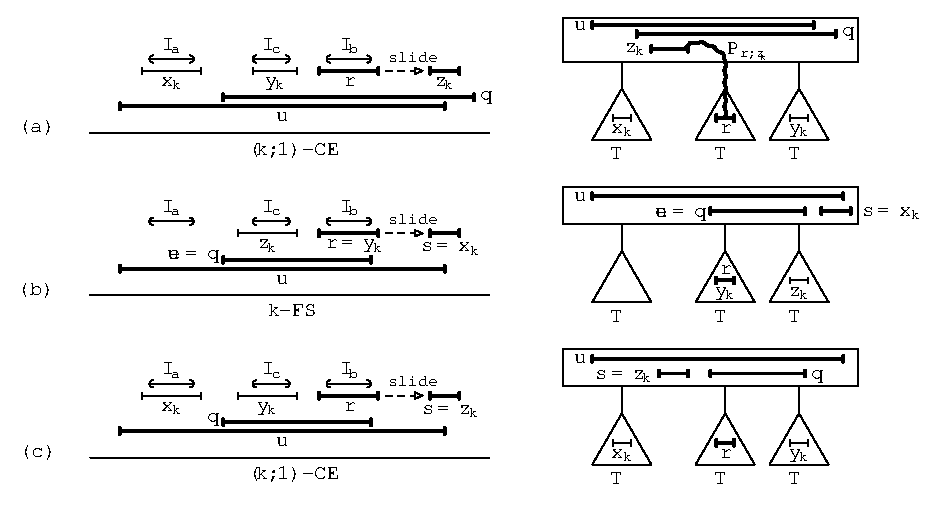
\includegraphics{q_nodes_q_and_r_case.eps}
\caption{Proof of Lemma~\ref{lem:q_node_q_and_r_case}. On the left, the pre-drawn
intervals. On the right, their positions in the MPQ-tree. (a) Case 1. (b) Subcase 2A. (c) Subcase 2B.}
\label{fig:q_nodes_q_and_r_case}
\end{figure}

\emph{Case 2: $q \in P^{\endlft}(c)$}. Then $r(q) < r(u)$.
First we argue that, without loss of generality, we can assume that either $\inter q'$ and $\inter
r'$ are disjoint, or $\inter r'$ covers $r(q)$. Suppose that $\inter r'$ is contained in $\inter
q'$. Since $q \in P^{\endlft}(c)$, this implies that $P(c) \subsetneq P(b)$. By applying Sliding
Lemma~\ref{lem:sliding} to $I_c$, $I_b$ and $r$, we obtain a pre-drawn interval $\widetilde r$ not
in $P(c)$ which covers $r(q)$.  We also get a path $P_{r,\widetilde r}$ whose vertices are
pre-drawn and not contained in $P(c)$; since $I_a$ is on the left of $I_c$, they are also not in $P(a)$.
Therefore $\widetilde r$ is between $a$ and $c$ in the Q-node. Further, $\widetilde r$ belongs to
some clique $\widetilde b$ for which $I_{\widetilde b}$ is on the right of $I_c$. From now on, we
work with $\widetilde r$ as $r$, and with $\widetilde b$ as $b$. Hence the
assumption on the relative positions of $\inter q'$ and $\inter r'$ holds.

We apply Sliding Lemma~\ref{lem:sliding} to $I_a$, $I_b$ and $r$, and we get a pre-drawn interval $s
\notin P(a)$ covering $r(u)$. This sliding is weaker that in Case 1: we know that $s$ is on the
right of $a$, but we do not know its position with respect to $c$.  We distinguish three subcases
according to the relative positions of $q$ and $s$ in the Q-node.

\emph{Subcase 2A: $s$ is on the right of $q$.}
The situation is depicted in Fig.~\ref{fig:q_nodes_q_and_r_case}b.  Let $x_k = s$ and $y_k = r$.  If
$\inter q'$ is on the left of $\inter r'$, let $z_k = q$. Otherwise, let $z_k \in c$ be a vertex
non-adjacent to $r$, but possibly adjacent to $x_k$.  Since in every extending
representation $z_k$ is placed on the left of $y_k$, we can apply $k$-FAT
Lemma~\ref{lem:k_fat} to $x_k$, $y_k$ and $z_k$, and get a subgraph $H_k$.  If $\inter q'$ is on the
left of $\inter r'$, then $H_k$ gives a $k$-FAT obstruction.  If $\inter r'$ covers $r(q)$, then
$H_k$ together with $\widetilde u = q$ gives a $k$-FS obstruction.

\begin{figure}[t!]
\centering
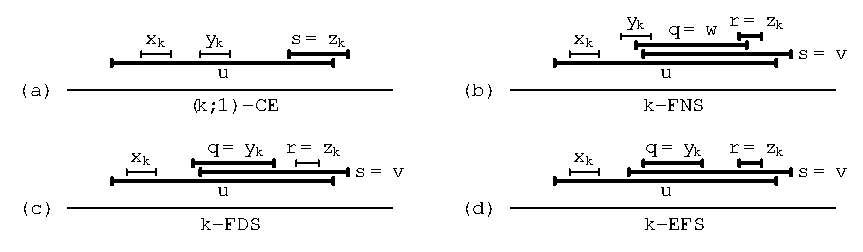
\includegraphics{q_nodes_q_and_r_case_obstructions.eps}
\caption{Four possible obstructions obtained in Subcase 2C of the proof of
Lemma~\ref{lem:q_node_q_and_r_case}. (a) If $s \notin P(c)$, we get a $(k,1)$-CE obstruction. (b) If
$\inter q'$ intersects $\inter r'$, we get a $k$-FNS obstruction. Recall that the relative order of
$\ell(q)$ and $\ell(s)$ does not matter. (c) If $\inter q'$ is on the left of $\inter r'$ and
$\ell(q) \le \ell(s)$, we get a $k$-FDS obstruction.  (d) If $\inter q'$ is on the left of $\inter
r'$ and $\ell(s) < \ell(q)$, we get a $k$-EFS obstruction.}
\label{fig:q_nodes_q_and_r_case_obstructions}
\end{figure}

\emph{Subcase 2B: $s$ is on the left of $q$.}
We choose $x_k \in a$ and $y_k \in c$ non-adjacent to $s$; such vertices exist because $s$ is
between $a$ and $c$ in the Q-node. By $(k,\ell)$-CE Lemma~\ref{lem:kl_ce}, we get a $(k,\ell)$-CE
obstruction for $x_k$, $y_k$, $z_k = s$ and $u$. Notice that we can construct a path
$P_{y_k,z_k}$ from $y_k$ to $z_k$ avoiding $N[x_k]$ by applying Sliding Lemma~\ref{lem:sliding} to
$I_a$, $I_c$, and $q$. Thus $\ell = 1$.

\emph{Subcase 2C: $\inter s'$ intersects $\inter q'$.}
Notice that $\inter s'$ also intersects $\inter r'$. Therefore, if $s \notin P(c)$, then it appears
in the Q-node between $a$ and $c$. Let $z_k = s$, we get a $(k,1)$-CE obstruction as follows.  We
choose $y_k \in c$ non-adjacent to $z_k$.  By Lemma~\ref{lem:non_adjacent}, there exists $x_k \in a$
non-adjacent to $q$, $y_k$, and $z_k$. By $(k,\ell)$-CE Lemma~\ref{lem:kl_ce}, we get a $(k,1)$-CE
obstruction for $x_k$, $y_k$, $z_k$ and $u$ as illustrated in
Fig.~\ref{fig:q_nodes_q_and_r_case_obstructions}a; notice that the path $y_kqz_k$ avoids $N[x_k]$.

It remains to deal with the situation when $s \in P(c)$.  Let $z_k = r$. If $\inter q'$ intersects
$\inter {r}'$, let $y_k \in c$ be a vertex non-adjacent to $r$; otherwise let $y_k = q$. By
Lemma~\ref{lem:non_adjacent}, there exists $x_k \in a$ non-adjacent to $q$, $y_k$, and $z_k$.  In
every extending representation, $\inter{y_k}$ is placed on the left of $\inter{z_k}'$, and
$\inter{x_k}$ is placed on the left of $\inter{y_k}$.  Therefore, by $k$-FAT Lemma~\ref{lem:k_fat},
we get a subgraph $H_k$ of a $k$-FAT obstruction.  Together with $u$, $v = s$, $w = q$ (for $y_k \ne
q$), or possibly some of them, we get a $k$-FDS, $k$-EFS, or $k$-FNS obstruction; see
Fig.~\ref{fig:q_nodes_q_and_r_case_obstructions}b, c, and d.\qed
\end{proof}

The case where $P(b) \subsetneq P(c)$ is addressed in Lemmas~\ref{lem:q_node_p_and_q_case}
and~\ref{lem:q_node_q_case}. First, we need an auxiliary result.

\begin{lemma} \label{lem:q_node_q_case_wlog}
If $I_a$ is on the left of $I_c$ and $P(b) \subsetneq P(c)$, there exist $q \in P(c) \setminus
P(b)$ and $r \in P(b) \setminus P(a)$ such that $\inter q'$ is on the right of $I_a$ and on the left
of $I_b$, and $\inter r'$ is on the right of $I_a$, containing $I_c$ and $I_b$.  Without loss of
generality, $\inter q'$ covers $\ell(r)$.
\end{lemma}

\begin{proof}
The proof is depicted in Fig.~\ref{fig:q_nodes_q_case_wlog}. Clearly, there exists $q \in P(c) \setminus
P(b)$. Due to the structure of the Q-node, we also have that $q \notin P(a)$.  Therefore, $\inter
q'$ is between $I_a$ and $I_b$. 

\begin{figure}[b!]
\centering
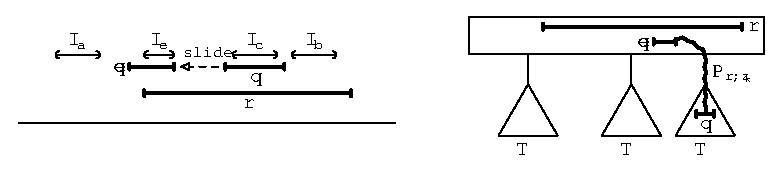
\includegraphics{q_nodes_q_case_wlog.eps}
\caption{Proof of Lemma~\ref{lem:q_node_q_case_wlog}. On the left, the pre-drawn
intervals. On the right, their positions in the MPQ-tree.}
\label{fig:q_nodes_q_case_wlog}
\end{figure}

Next, we argue that there exists $r \in P(b) \setminus P(a)$. For contradiction, assume that $P(b)
\subsetneq P(a)$. Let $v \in P^{\startrt}(b)$; notice that $v$ contains $I_a$ and $I_c$. By the
flipped version of Sliding Lemma~\ref{lem:sliding} applied to $I_c$, $I_b$ and $q$, there exists a
path consisting of pre-drawn intervals not contained in $P(b)$ from $q$ to $z$, where $\inter z'$
covers $\ell(v)$. At least one interval of this path intersects $I_a$, so it belongs to $P(a)$. This
contradicts the fact that $b$ is between $a$ and $c$ in the Q-node. Hence, there exists $r \in P(b)
\setminus P(a)$.

We choose $r$ having rightmost left endpoint. Clearly, $\inter r'$ is on the right of $I_a$, and
contains $I_b$ and $I_c$. Suppose that $\ell(r) < \ell(q)$. Since $r$ has  rightmost left endpoint
among all intervals in $P(b) \setminus P(a)$, and every interval in $P(a)$ has its left endpoint
more to the left, we obtain that $r \in P^{\startrt}(b)$. Therefore, we can apply the flipped
version of Sliding Lemma~\ref{lem:sliding} to $I_c$, $I_b$ and $q$. We get a pre-drawn interval
$\widetilde q \notin P(b)$ covering $\ell(r)$, and a path $P_{q,\widetilde q}$ from $q$ to
$\widetilde q$ whose vertices are not in $b$.  Therefore, $\widetilde q$ is on the right of $b$ in
the Q-node. Let $\widetilde c$ be a maximal clique containing $\widetilde q$. Since $I_{\widetilde
c}$ is contained in $\widetilde q$, it is between $I_a$ and $I_b$. Therefore, we can work with
$\widetilde q$ and $\widetilde c$ instead of $q$ and $c$. Thus we can assume that $\inter q'$ covers
$\ell(r)$.\qed
\end{proof}

For $P(b) \subsetneq P(c)$, we distinguish two cases.

\begin{lemma} \label{lem:q_node_p_and_q_case}
If $I_a$ is on the left of $I_c$, $P(b) \subsetneq P(c)$, and $P(a) \setminus P(c) \ne
\emptyset$, then $G$ and $\calR'$ contain a $k$-FS obstruction.
\end{lemma}

\begin{proof}
The proof is illustrated in Fig.~\ref{fig:q_nodes_p_and_q_case}. By Lemma~\ref{lem:q_node_q_case_wlog}, there exist $q \in P(c) \setminus
P(b)$ and $r \in P(b) \setminus P(a)$ such that $\inter q'$ covers $\ell(r)$. Let $x_k \in P(a) \setminus P(c)$
and $y_k = q$. Then $\inter{x_k}'$ is on the left of $I_c$, and therefore also on the left of $I_b$. Thus
$x_k \notin P(b)$. We infer that $x_k$ is on the left of $b$ in the Q-node, so it is non-adjacent to
$y_k$. In consequence, $\inter{x_k}'$ is on the left of $\inter{y_k}'$. Let $z_k \in b$ be a vertex
non-adjacent to $y_k$. 

\begin{figure}[t!]
\centering
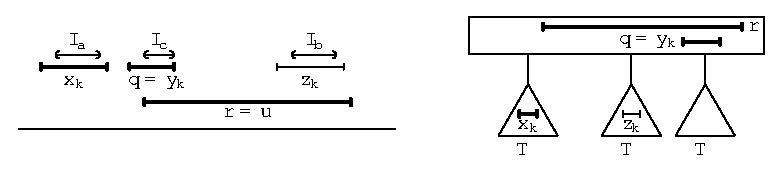
\includegraphics{q_nodes_p_and_q_case.eps}
\caption{Proof of Lemma~\ref{lem:q_node_p_and_q_case}. We derive that $\inter{x_k}'$ is on the
left of $\inter q'$, which gives a $k$-FS obstruction based on the positions in the Q-node.}
\label{fig:q_nodes_p_and_q_case}
\end{figure}

If $z_k$ is adjacent to $x_k$, we get a $1$-FS obstruction.  Otherwise, in every extending
representation, $\inter{z_k}$ is to the right of $\inter{y_k}'$.  By $k$-FAT
Lemma~\ref{lem:k_fat}, we get a subgraph $H_k$ of a $k$-FAT obstruction.  Together with $u = r$,
this leads to a $k$-FS obstruction.\qed
\end{proof}

\begin{lemma} \label{lem:q_node_q_case}
If $I_a$ is on the left of $I_c$, $P(b) \subsetneq P(c)$ and $P(a) \subsetneq P(c)$, then $G$ and $\calR'$ contain a
$(k,1)$-CE, $k$-FB, $k$-BI, $k$-FDS, or $k$-EFDS obstruction.
\end{lemma}

\begin{proof}
Let $p \in P^{\endlft}(a)$, and $q$ be the vertex from Lemma~\ref{lem:q_node_q_case_wlog}. By
applying Sliding Lemma~\ref{lem:sliding} to $I_a$, $I_c$ and $q$, we get a pre-drawn interval $s
\notin P(a)$ covering $r(p)$, and path $P_{q,s}$ of intervals not in $P(a)$, so $s$ appears on the
right of $a$ in the Q-node.  Similarly, as in Case 2 of the proof of
Lemma~\ref{lem:q_node_q_and_r_case}, we distinguish three cases according to the relative positions
of $s$ and $q$ in the Q-node; see Fig~\ref{fig:q_nodes_q_case}.

\begin{figure}[t!]
\centering
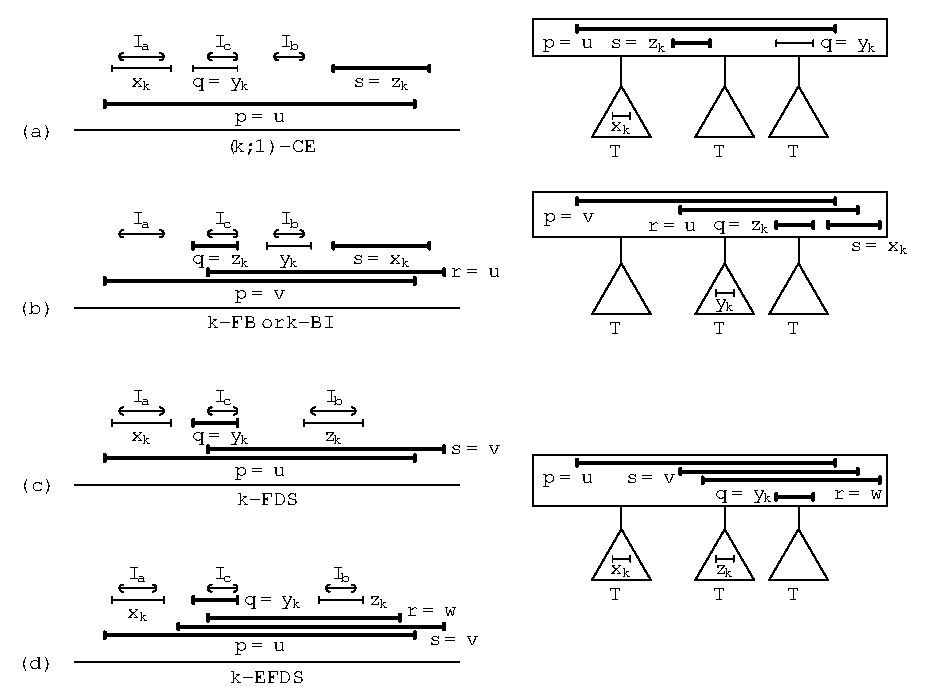
\includegraphics{q_nodes_q_case.eps}
\caption{Proof of Lemma~\ref{lem:q_node_q_case}. On the left, the pre-drawn
intervals. On the right, their positions in the MPQ-tree. (a) Case 1. (b) Case 2. (c) Case 3, if
$\ell(y_k) \le \ell(s)$. (d) Case 3, if $\ell(y_k) > \ell(s)$.}
\label{fig:q_nodes_q_case}
\end{figure}

\emph{Case 1: $s$ is on the left of $q$.} By Lemma~\ref{lem:non_adjacent}, there exists $x_k \in a$
non-adjacent to all vertices of $P_{q,s}$, in particular non-adjacent to $s$ and $q$.  Let $y_k =
q$, $z_k = s$, and $u = p$.  Clearly, $z_k$ is between $x_k$ and $y_k$ in the Q-node. By
$(k,\ell)$-CE Lemma~\ref{lem:kl_ce} and the existence of $P_{y_k,z_k}$, we get a $(k,1)$-CE
obstruction. Notice that $\inter{y_k}'$ can be made free; see Fig.~\ref{fig:q_nodes_q_case}a.

\emph{Case 2: $s$ is on the right of $q$.} Since $q$ is between $b$ and $s$ in the Q-node, we get
that $s \notin P(b)$. Let $x_k = s$, $z_k = q$, and $u = r$, where $r$ is the vertex from
Lemma~\ref{lem:q_node_q_case_wlog}. There exists $y_k \in b$ non-adjacent to $z_k$ and, by the
structure of the Q-node, also non-adjacent to $x_k$.  Since $y_k$ is adjacent to $p$ and $r$,
$\inter{y_k}$ is between $\inter{x_k}'$ and $\inter{z_k}'$ in every extending representation.  By
$k$-FAT Lemma~\ref{lem:k_fat}, we get a subgraph $H_k$ of a $k$-FAT obstruction.  If $r(r) \le
r(x_k)$, together with $u$, we obtain a $k$-FB or a $k$-BI obstruction. If $r(r) > r(x_k)$, together
with $u$ and $v=p$, we obtain a $k$-BI obstruction; see Fig.~\ref{fig:q_nodes_q_case}b.

\emph{Case 3: $\inter s'$ intersects $\inter q'$.}
Since $s$ contains $I_b$, it belongs to $P(b)$. Let $y_k = q$, $u = p$, $v = s$, and $w = r$; we
note that possibly $s=r$.  By Lemma~\ref{lem:non_adjacent}, there exists $x_k \in a$ non-adjacent to
$y_k$, $v$, and $w$. Since $x_k$ is adjacent to $u$, then $\inter{x_k}$ is on the left of
$\inter{y_k}'$ in every extending representation. Finally, there exists $z_k \in b$ non-adjacent to
$y_k$. Since $z_k$ is adjacent to $u$, $v$, and $w$, we have that $\inter{z_k}$ is on the right of
$\inter{y_k}'$ in every extending representation.

Since $z_k$ is between $x_k$ and $y_k$ in the Q-node, we can apply $k$-FAT Lemma~\ref{lem:k_fat},
which gives a subgraph $H_k$ of a $k$-FAT obstruction.  If $\ell(y_k) \le \ell(v)$, together with
$u$ and $v$, we obtain a $k$-FDS obstruction; see Fig.~\ref{fig:q_nodes_q_case}c. If $\ell(y_k) >
\ell(v)$, together with $u$, $v$, and $w$, we get a $k$-EFDS obstruction; see
Fig.~\ref{fig:q_nodes_q_case}d.\qed
\end{proof}

In summary, we conclude:

\begin{lemma}[The Q-node, Three Subtrees] \label{lem:q_node_three}
If the three cliques creating the obstruction belong to three different subtrees, then $G$ and
$\calR'$ contain a $k$-FAT, $k$-BI ($k \le 2$), $k$-FS, $k$-EFS, $k$-FB, $k$-EFB, $k$-FDS,
$k$-EFDS, $k$-FNS, or $(k,\ell)$-CE obstruction (either $k=\ell=2$, or $k \ge \ell = 1$).
\end{lemma}

\begin{proof}
For an overview, see the diagram in Fig.~\ref{fig:q_nodes_three_subtrees_diagram}. The proof follows
from Lemmas~\ref{lem:q_node_wlog_lemma}, \ref{lem:q_node_containment_case},
\ref{lem:q_node_p_and_r_case}, \ref{lem:q_node_q_and_r_case}, \ref{lem:q_node_q_case_wlog},
\ref{lem:q_node_p_and_q_case}, and \ref{lem:q_node_q_case}.\qed
\end{proof}
